\label{chap3}

This chapter details the parameter identification of the soft robotic actuator. First, material properties and dimensions of the soft robotic manipulator are provided. Then, determination of actuator stiffness for elongation and curvature explained. Consequently, pressure to force input mapping is detailed. At this point it should be emphasized that during experimental analysis the soft actuator, on which this parameter study is based, was too porous. This allowed too much air to escape and therefore was not suitable for further use. Therefore, the methodology of acquiring stiffness data and pressure mapping should be valued instead of found parameters. During experimental analysis a geometric equivalent planar actuator is used. 


Parameter identification is necessary for model simulation as well as experimental validation. Key actuator parameters such as actuator mass and dimensions were presented in an earlier work \cite{berkers}. Since the robotic manipulator is manufactured by an external company, some material properties are classified. To our best knowledge, the Young's Modulus and Poisson ratio are equal to those presented in Table (\ref{tab4:parameters}). These properties allow to calculate shear modulus $\mu$ as $\frac{E}{2(1+\nu)}$ and bulk modulus $\kappa$ as $\frac{E}{3(1-2\nu)}$. It is assumed that the robotic manipulator deforms non-linearly following Neo-Hookeon behaviour \cite{Caasenbrood2020StiffnessModel}. For consistency with linear elasticity these moduli are reformulated as $C_{10} = \frac{\mu}{2}$ and $D_{1} = \frac{2}{\kappa}$ as used for Finite Element Analysis (FEA) \cite{neohookean}. The geometrical properties are presented in Figure \ref{fig3:dim}.


\begin{table}[H]
    \centering
    \caption{Actuator properties}
    \begin{tabular}{|c|c|c|} \hline
      \textbf{Parameter}   &  \textbf{Value} & \textbf{Unit} \\ \hline
      Mass $m$             &    0.0332       & $[kg]$ \\ 
      Nominal length $L_0$ &    0.0644       & $[m]$  \\ 
      Actuator width  $w$     &    0.0664       & $[m]$  \\
      Lever length $r$     &    0.01256      & $[m]$  \\ 
      Young's Modulus $E$  &    69           & $[MPa]$\\ 
      Poisson ration $\nu$ &    0.45         & $[-]$ \\ \hline
    \end{tabular}
    \label{tab4:parameters}
\end{table}

\begin{figure}[H] 
    \begin{minipage}[b]{0.49\linewidth}
     \centering
    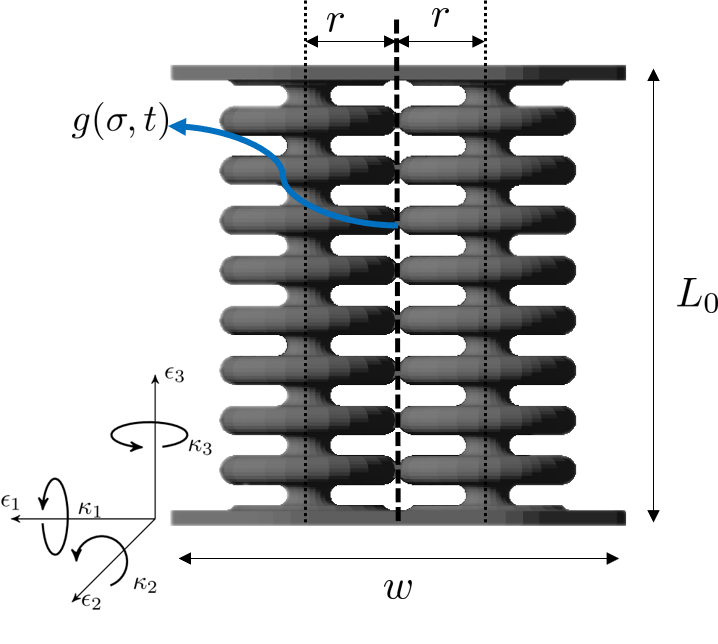
\includegraphics[width=\linewidth]{Figures/Chapter3/dimensions.png} 
    \caption{Schematic overview of the undeformed actuator with its dimensions.} 
    \label{fig3:dim} 
       \end{minipage} 
    \begin{minipage}[b]{0.49\linewidth}
     \centering
    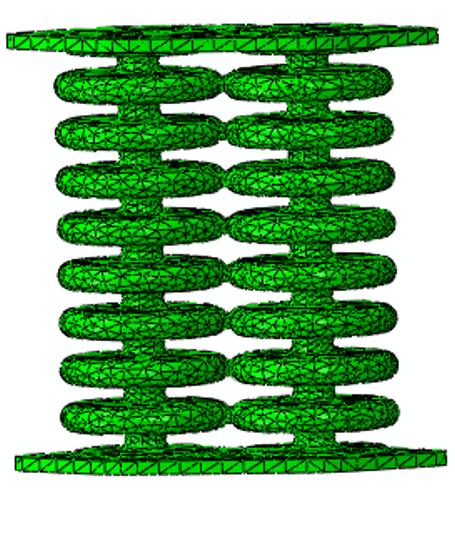
\includegraphics[width=0.7\linewidth]{Figures/Chapter3/undeformed2.png} 
    \caption{Undeformed meshed Finite Element model of the planar actuator.} 
    \label{fig3:FemModel} 
    \end{minipage} 
\end{figure}

%%%%%%%%%%%%%%%%%%%%%%%%%%%%%%%%%%%%%%%%%%%%%%%%%%%%%%%%%%%%%%%%%%%%%%%%
%%%%%%%%%%%%%%%%%%%%%%%%%%%%%%%%%%%%%%%%%%%%%%%%%%%%%%%%%%%%%%%%%%%%%%%%
%%%%%%%%%%%%%%%%%%%%%%%%%%%%%%%%%%%%%%%%%%%%%%%%%%%%%%%%%%%%%%%%%%%%%%%%

\section{Finite Element Analysis (FEA)}

In an effort to determine stiffness properties, finite element software \verb+Abaqus/CAE+ is used. This software allows to study deformation of the actuator under various loads. Stiffness can be approximated by relating applied forces to the magnitude of deformation. Here we want to relate pressure, thus its resulting force, to induced elongation and curvature. Figure  \ref{fig3:FemModel} shows the meshed model used in the finite element software. A mesh refinement analysis is done to determine an accurate mesh size, see Appendix \ref{app:chap3}. In the analysis, the bottom plate of the actuator is constrained in all directions of motion and rotation. Furthermore, the out-of-plane motion of the actuator is not considered since the body is symmetric, and applied loads act perpendicular to this motion. Also, gravitational effects are omitted. Lastly, the following assumption is made. 

\begin{theorem}
The actuator is assumed to be symmetrical along its longitudinal axis. Both bellows therefore deform uniformly.
\end{theorem}


In this finite element analysis we only consider the curvature induced by pressurizing a single bellow. Due to symmetry we assume that inflating the other bellow will result in equal rotation but in opposite direction. Two different analysis are performed. The first analysis focuses on curvature, the second analysis targets elongation. 


\subsection{Curvature analysis}

The curvature analysis allows to determine rotation stiffness of the robot manipulator. For this analysis only a single bellow is pressurized, while the other bellow pressure is kept zero. The force created by this pressurized bellow causes a moment around the center of the actuator. This will case the actuator to curve and elongate. Figure \ref{fig3:schematiccurvature} shows the deformation the actuator undergoes during a curvature simulation. Here the undeformed actuator is visualized in blue. For the black actuator the left bellow is pressurized to 60 kPa.


After applying loads to the finite element model, nodal displacements by can be outputted from $\verb+Abaqus+$. The acquired data is post-processed in \MATLAB to estimate the elongation and curvature. A post-proccessed image of the deformation is shown in Figure \ref{fig3:nodalcurvatrue}. This image is created by isolating specific nodes, necessary to reconstruct the backbone curve. In this figure, top and bottom plate of the actuator are clearly visible. Using \MATLAB function \verb+affine_fit.m+ \cite{affinefit} the orientation of both planes with their normal vector can be obtained. Furthermore, this function determines the weighted average of all nodes of the top plate. Which coincides with the end-effector position of the actuator. Lastly, the nodes that are situated at the exact geometrical mid over the longitudinal axis are isolated. These clusters of nodes are used to reconstruct the backbone curve. 


The post-processed image can be used for kinematic model fitting. This is the last step to obtain modal coordinates $\epsilon$ and $\kappa$ from the finite element simulation. Figure \ref{fig3:nodalfitcurv} shows this kinematic model fit. Here the black cross again indicates the end-effector position. Initially, the kinematic fitting is done with the aid of the developed inverse kinematic model as detailed in Appendix \ref{app:chap2}. An inverse kinematic solution can be found based on the end-effector position and rotation. The solution to this kinematic fitting procedure is indicated by the purple curve. This result was deemed insufficiently accurate. Therefore an optimization method is proposed. This optimization method takes into account the curvature of the entire backbone curve. For each cluster of nodes among the backbone the weighted average is calculated. Those are indicated with a blue cross and denoted as vector $\Bar{x}_{mid} \in \mathbb{R}^{2\times N}$. Furthermore, the length of the backbone curve is determined using the function \verb+arc_length.m+ \cite{arclength}. This functions uses vector $\Bar{x}_{mid}$ to approximate the arc length using splines. This estimated arc length is represented as  $\Bar{x}_{length} \in \mathbb{R}^+ $. The optimization is done via optimization with \verb+fmincon.m+. The minimization problem that follows is,


\begin{equation}
\begin{aligned}
\min_{q} \hspace{5pt}  q^\top Q q  + \sum_{i=1}^{N}[\Phi_1(\Bar{x}_{mid} - f(q))^2] +   \Phi_2(\Bar{x}_{end}  - f(q)_{end})^2 +  \Phi_3(\Bar{x}_{length} - & f(q)_{length})^2  \\ 
\text{s.t.} \hspace{5pt} \epsilon - 1 > 0
\end{aligned}
\label{eq3:optim}
\end{equation}


where $Q$ is $\text{diag}([0.01,1])$ is a weighing matrix used to penalize the value of the modal coordinates. Additional weighing factors $\Phi_i \in \mathbb{R}^+$ and $i \in \{1,2,3\}$ are applied to penalize individual terms and equal to $1e5$,$1e5$ and $5e4$, respectively. The imposed constrained affects the elongation of the manipulator. Physically this constraint implies that the actuator can shorten in length, but the length can not become negative. The modal coordinates find through optimization for this simulation are $q = [\kappa,\epsilon]^\top = [14,0.24]^\top$.


Above described inverse kinematic optimization is ran for multiple finite element analysis conducted various pressures. The results are displayed in Figure \ref{fig3:rotationvspressure}. Here the obtained curvature and elongation are plotted as a function of bellow pressure. It can be seen that the curvature and elongation rates increase by increments in pressure. Also the non-linear relation between pressure and deformation is visible.

\begin{figure}[H]
    \centering
\begin{minipage}{0.5\textwidth}
        \centering
        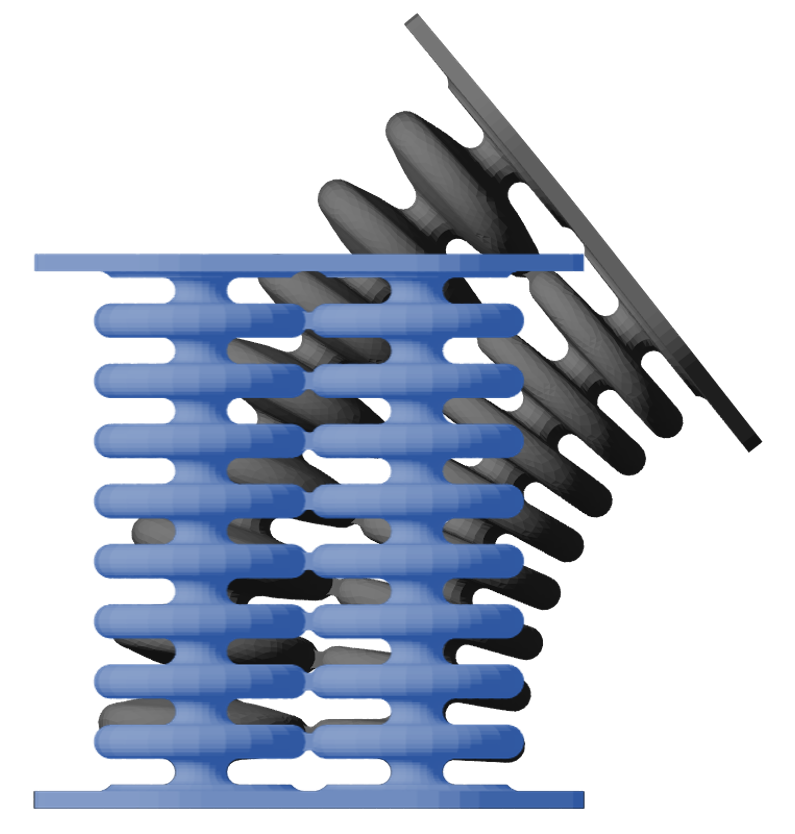
\includegraphics[width=0.695\textwidth]{Figures/Chapter3/curvature.png} 
        \caption{Curvature analysis, undeformed actuator blue and deformed actuator for curvature experiment. }
        \label{fig3:schematiccurvature}
    \end{minipage}\hfill
    \begin{minipage}{0.5\textwidth}
        \centering
        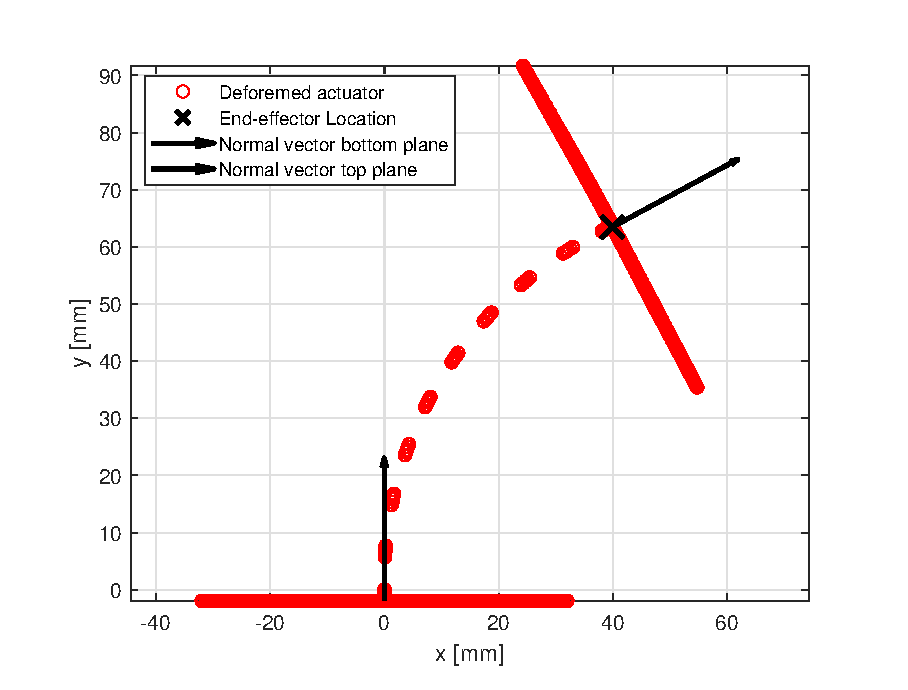
\includegraphics[width=\textwidth]{Figures/Chapter3/rotation60kpa.eps} 
        \caption{Post-processed image of the curvature analysis. The nodes that form the backbone curve clearly isolated.}
        \label{fig3:nodalcurvatrue}
    \end{minipage}
\begin{minipage}{0.5\textwidth}
        \centering
        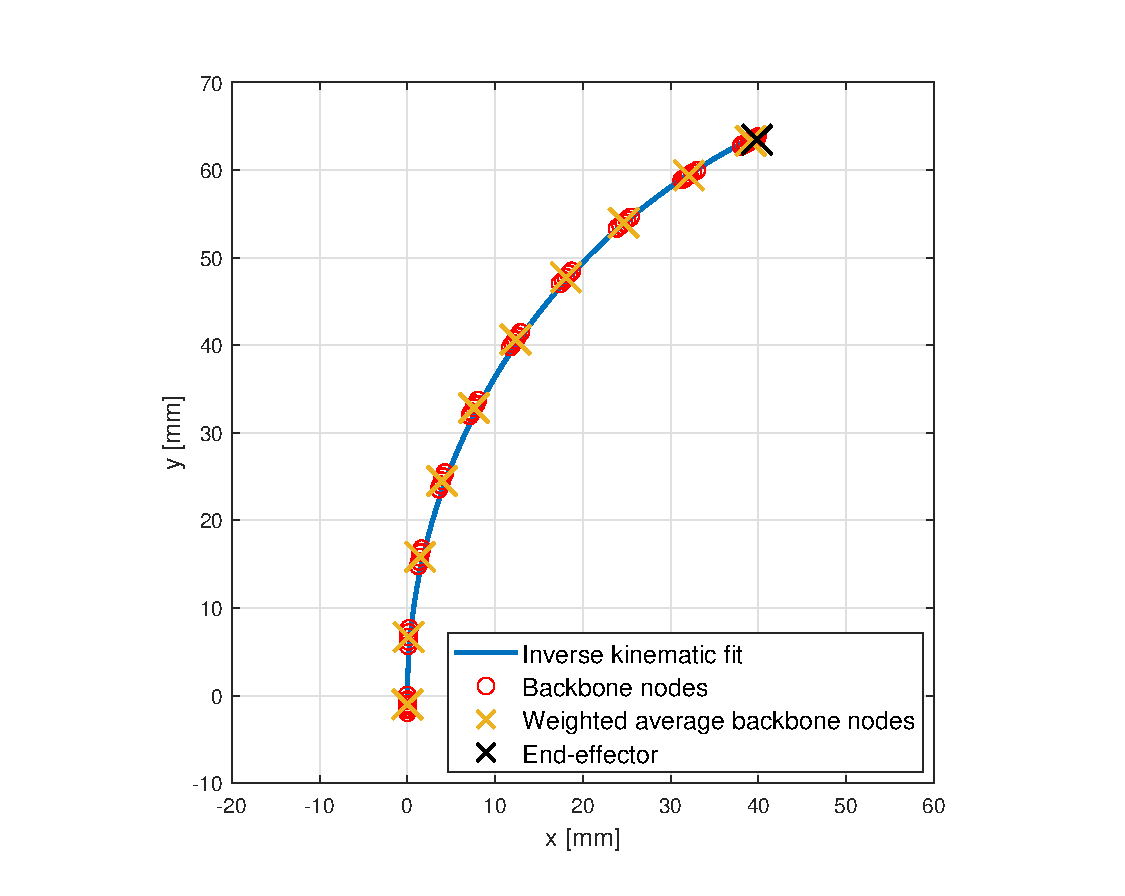
\includegraphics[width=\textwidth]{Figures/Chapter3/nodalfit.eps}
        \caption{Inverse kinematic fit for an elongation analysis. Both bellows pressurized to 60kPa.}
        \label{fig3:nodalfitcurv}
    \end{minipage}\hfill
    \begin{minipage}{0.5\textwidth}
        \centering
        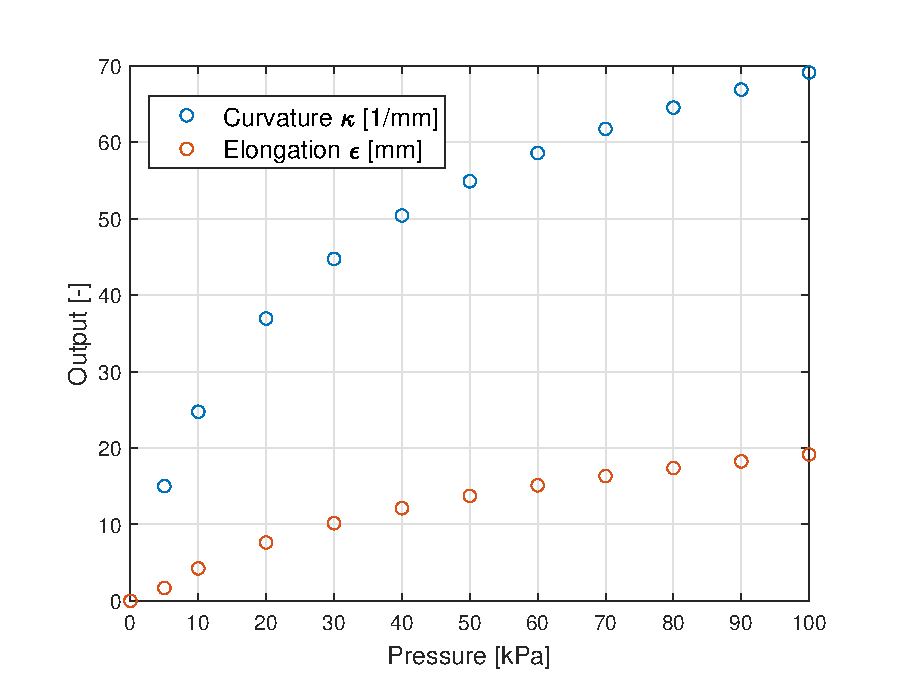
\includegraphics[width=\textwidth]{Figures/Chapter3/rotationvspressure.eps} 
        \caption{Curvature analysis, elongation and curvature as function of pressure.}
        \label{fig3:rotationvspressure}
    \end{minipage}
\end{figure}






\subsection{Elongation analysis}


The elongation analysis aims to measure pure elongation of the soft actuator. This allows for determining elongation stiffness, as rotating effects of the top of the robot are small. ``Pure'' elongation is induced by pressurizing both bellows equally. Figure \ref{fig3:schematicelong} shows the deformation the actuator undergoes during an elongation experiment. Here the undeformed actuator is visualized in blue. For the black actuator both bellows are pressurized to 60 kPa. 

As for the curvature analysis, a post-processed image of the deformation is shown in Figure \ref{fig3:nodalelong}. The optimization of (\ref{eq3:optim}) is carried out, to determine modal coordinates. The results of this optimization is shown in Figure \ref{fig3:nodalfitelong}. The modal coordinates belonging to this fit are  $q = [\kappa,\epsilon] = [0.06, 0.45]^\top$, showing a negligible curvature. Furthermore, this figure shows that for elongation analysis, the developed inverse kinematic algorithm (Appendix \ref{app:chap2}) already yields decent results.  

Repeating this experiment for a set of pressures, a relation between elongation and pressure can be found. Figure (\ref{fig3:elongationvspressure}) shows the relation between elongation function of pressure. Additionally, the curvature of the manipulator is shown for various pressures. It can be seen that pressurizing the bellows equally results in a near pure elongation. The maximum obtained curvature is equal to 0.07 [1/m], which is equivalent to a rotation of around 0.32 degrees. This allows to determine the elongation stiffness as effects of rotation are deemed negligible. The elongation rate decreases as pressure increases, this is the result of a non-linear material parameters. As a remark, the found elongation for the elongation analysis is about double to those found for curvature analysis. For instance, the found elongation for the elongation experiment at 90 kPa is $0.55$, whereas for the curvature analysis the elongation at this pressure is $0.27$. This observation tells that the curvature and elongation are largely decoupled.




\begin{figure}[H]
    \centering
\begin{minipage}{0.5\textwidth}
        \centering
        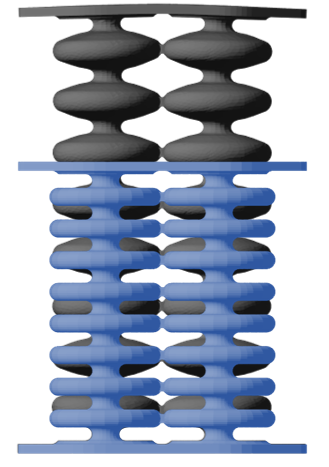
\includegraphics[width=0.53\textwidth]{Figures/Chapter3/elongation.png} 
        \caption{Elongation analysis, elongation and curvature as function of pressure. As can be seen curvature is negligibly small. }
        \label{fig3:schematicelong}
    \end{minipage}\hfill
    \begin{minipage}{0.5\textwidth}
        \centering
        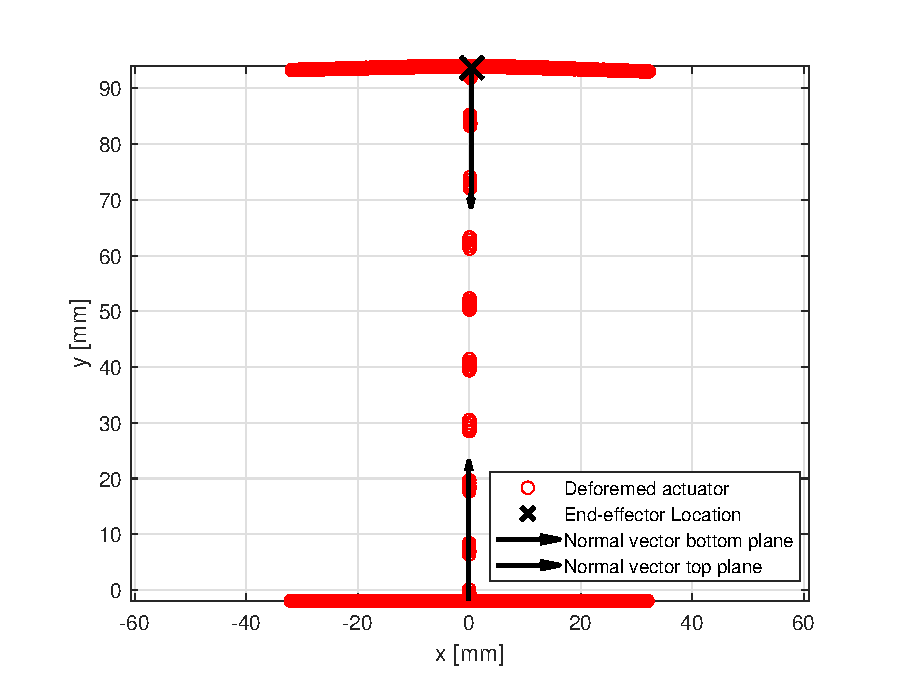
\includegraphics[width=\textwidth]{Figures/Chapter3/elongation60good.eps} 
        \caption{Post-processed image of an elongation analysis. The nodes that form the backbone curve clearly isolated.}
        \label{fig3:nodalelong}
    \end{minipage}
\begin{minipage}{0.5\textwidth}
        \centering
        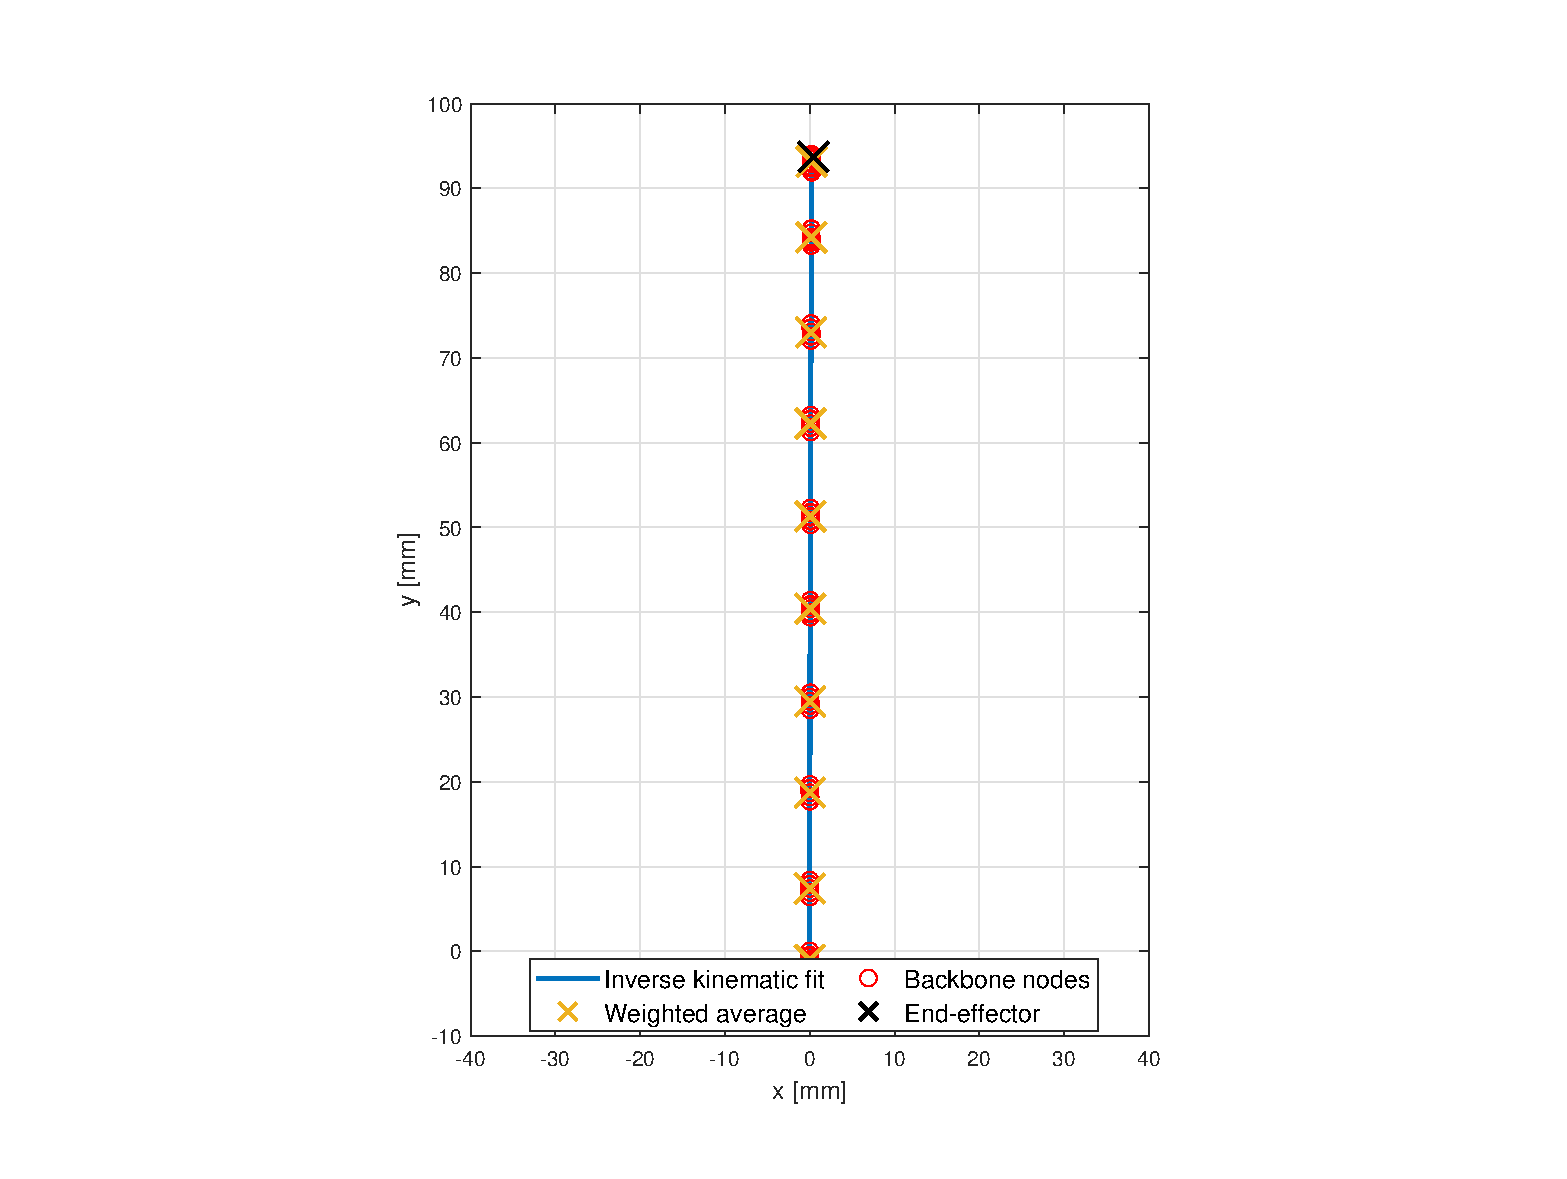
\includegraphics[width=\textwidth]{Figures/Chapter3/nodalfitelong.eps}
        \caption{Inverse kinematic fit for an elongation analysis. Both bellows pressurized to 60kPa.}
        \label{fig3:nodalfitelong}
    \end{minipage}\hfill
    \begin{minipage}{0.5\textwidth}
        \centering
        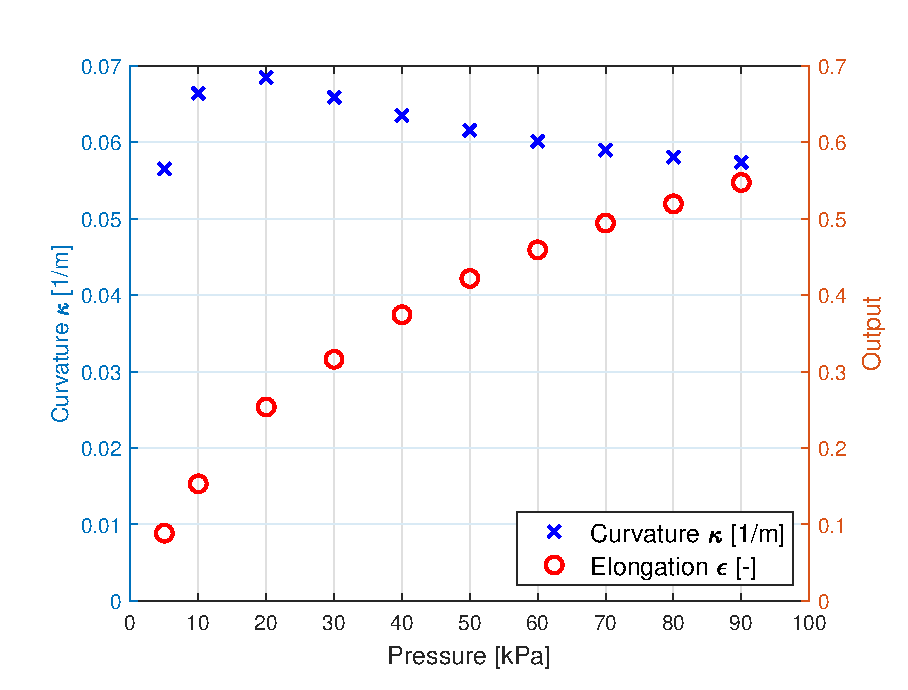
\includegraphics[width=\textwidth]{Figures/Chapter3/elongationvspressure.eps} 
        \caption{Elongation analysis, elongation and curvature as function of pressure. As can be seen curvature is negligibly small.}
        \label{fig3:elongationvspressure}
    \end{minipage}
\end{figure}

\newpage


At this point we have derived modal coordinates as function pressure. However, to determine the stiffness this pressure needs to be mapped to force and moment. This is discussed in Section \ref{sec3:InputMapping}.


\hl{adapt some figure axis,explain $f(q)$ in optimization problem, weigh factors}

%%%%%%%%%%%%%%%%%%%%%%%%%%%%%%%%%%%%%%%%%%%%%%%%%%%%%%%%%%%%%%%%%%%%%%%%
%%%%%%%%%%%%%%%%%%%%%%%%%%%%%%%%%%%%%%%%%%%%%%%%%%%%%%%%%%%%%%%%%%%%%%%%
%%%%%%%%%%%%%%%%%%%%%%%%%%%%%%%%%%%%%%%%%%%%%%%%%%%%%%%%%%%%%%%%%%%%%%%%



\section{Input Mapping}
\label{sec3:InputMapping}

Stiffness is the ratio between applied force and elongation. To determine stiffness for elongation and curvature, applied forces and direction of deformation is necessary. For the physical set-up, individual bellow pressure $p_i \in \mathbb{R}^{\geq 0}$ with $i$ $\mathbb{N} \in \{1,2\}$ can be regulated. Therefore force input vector $\tau$ is mapped to pressure by some mapping matrix $H \in \mathbb{R}^{2 \times 2}$. The relation between force input and pressure is given as, 

\begin{equation}
   \tau =   \begin{bmatrix} M \\ F \end{bmatrix}     = \underbrace{\begin{bmatrix}  a_1 & a_2 \\ a_3 & a_4 \end{bmatrix}}_{H}         \begin{bmatrix}  p_1 \\ p_2 \end{bmatrix}, \label{eq3:H}
\end{equation}

where entries of $H$ are to be determined. Our aim is to decouple rotation and elongation. Therefore, it is important to understand that $F$ causes elongation of the soft robotic actuator. Whereas, $M$ results in a curvature of the actuator. Therefore, the entries of $a_3$ and $a_4$ represent an effective surface area on which the pressure acts. Constant $a_1$ and $a_2$ represent a combination of effective surface area and lever on which the force acts. Due to symmetry properties it must hold that $a_1 = a_3$ and $a_1 = -a_2$.

First, the relation between pressure and force tried to be obtained. This will be done by using finite element software as mentioned. The idea is to map pressure to force by using elongation. Pressurizing both bellows equally, resulted in almost ``pure" elongation. Effectively, the same deformation can be achieved by applying an equally distributed force on the top plate of the actuator. To this end, simulations for a set of forces applied to the top of actuator are simulated. The results for this simulation are presented in Figure (\ref{fig3:forcemap}). The horizontal axis show the modal coordinates, determined using the inverse kinematic fit as discussed previously. The contribution to the curvature is for both pressure and force simulation comparable. The scaling of the of the vertical axis already reveals that a linear relation can be found.
\newpage

\begin{figure}[H]
    \centering
\begin{minipage}{0.5\textwidth}
        \centering
        \includegraphics[width=\textwidth]{Figures/Chapter3/forcepressuremodal.eps}
        \caption{Modal coordinates $\kappa$ and $\epsilon$ for elongation analysis and force analysis.}
        \label{fig3:forcemap}
    \end{minipage}\hfill
    \begin{minipage}{0.5\textwidth}
        \centering
        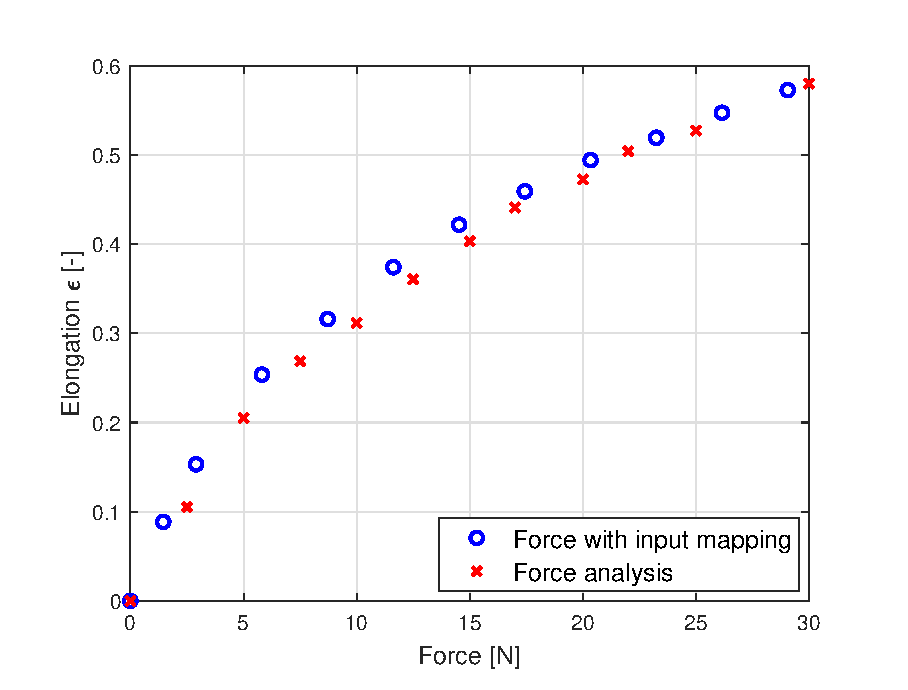
\includegraphics[width=\textwidth]{Figures/Chapter3/pressureforceelongation.eps} 
        \caption{Elongation expressed for force analysis and force with input mapping.}
        \label{fig3:forcetopressure}
    \end{minipage}
\end{figure}

The linear mapping coefficient, can be found by solving least squares problem as,

\begin{equation}
\min_{a_1} \sum_{i=1}^{N} (F_i - 2 a_1 p_i)^2
\label{eq3:forcefitting}
\end{equation}

where $i$ indicates each sample point. The effective pressure area is found to be equal to 0.1462. Since $a_3 = a_4$ the mapping of pressure in kPa to force in Newton is obtained. Figure (\ref{fig3:forcetopressure}) shows the results of the input mapping for the elongation. It can be seen that the pressure maps fairly accurate to the force.

Now the effective pressure area has been determined, the mapping to the moment can be calculated. It is assumed that the force acts on the top plate at a given radius form the backbone curve. The lever on which the force acts is equal to 12.56 mm, as can be seen in Figure \ref{fig3:dim}. This allows to calculate $a_1$ and $a_2$ by multiplying $a_3$ with this distance. The mapping matrix $H$ then follows as,

\begin{equation}
    H =  \begin{bmatrix} 1.8245e-3 & -1.8245e-3 \\
    0.14526 & 0.14526\end{bmatrix}  
\end{equation}


%%%%%%%%%%%%%%%%%%%%%%%%%%%%%%%%%%%%%%%%%%%%%%%%%%%%%%%%%%%%%%%%%%%%%%%%
%%%%%%%%%%%%%%%%%%%%%%%%%%%%%%%%%%%%%%%%%%%%%%%%%%%%%%%%%%%%%%%%%%%%%%%%
%%%%%%%%%%%%%%%%%%%%%%%%%%%%%%%%%%%%%%%%%%%%%%%%%%%%%%%%%%%%%%%%%%%%%%%%



\section{Stiffness properties}

The force mapping and the modal coordinates obtained through inverse kinematic optimization can be used to determine elongation and curvature stiffness. A non-linear trend in elongation and curvature as function of pressure was already observed. Therefore, it is assumed that the stiffness can be captured by the hyper-elastic stiffness model as formulated in \cite{Caasenbrood2020StiffnessModel}. This non-linear stiffness model poses that stiffness $k(q_i) \in \mathbb{R}^{\geq 0}$ and meets condition $\underbar{$k$} < k(q_i) < \Bar{k}$. The model used to describe elongation is described by,

\begin{equation}
    K_\epsilon(\alpha,q_\epsilon) =  \alpha_1 + \alpha_2 [\tanh({\alpha_3 \epsilon})^2 -1]
\end{equation}


where $\alpha_i$ and  for $i \in \{1,2,3\} $ are positive stiffness parameters to be found. It is assumed that negative pressures, e.g. creating a vacuum, result in equal elongation yet in opposite direction. Hence, self contact of the bellows is neglected. This assumption is deemed valid since this situation can not occur in our experimental set-up. The pumps used for experimental validation can not create vacuum. These stiffness parameters can be found by solving the non linear constraint optimisation described by,


\begin{equation}
\begin{aligned}
\min_{\alpha_1,\alpha_2,\alpha_3} \hspace{5pt} \sum_{i=1}^{N}(F_i -  (\alpha_1 + \alpha_2 [\tanh({\alpha_3 \epsilon_i})^2 -1])\epsilon_i)^2    \\ 
\text{s.t.} \hspace{5pt} \alpha_1 > \alpha_2 > 0 \\
\alpha_3 > 0 \\ 
\label{eq3:Keopt}
\end{aligned}
\end{equation}

which objective is to minimize the the sum of the errors between the mapped force, and force resulting from the stiffness model. As for the elongation stiffness, the curvature stiffness can be characterized by,

\begin{equation}
    K_\kappa(\beta,q_\kappa) =  \beta_1 + \beta_2 [\tanh({\beta_3 \kappa})^2 -1]
\end{equation}


where $\beta_i$ for $i \in \{1,2,3\} $ are positive stiffness parameters to be found. These parameters can be found by solving,

\begin{equation}
\begin{aligned}
\min_{\beta_1,\beta_2,\beta_3} \hspace{5pt} \sum_{i=1}^{N}(M_i -  (\beta_1 + \beta_2 [\tanh({\beta_3 {\kappa_i}})^2 -1]){\kappa_i})^2    \\ 
\text{s.t.} \hspace{5pt} \beta_1 > \beta_2 > 0 \\
\beta_3 > 0 \\ 
\label{eq3:Kkopt}
\end{aligned}
\end{equation}



where the objective is to minimize the sum of errors between the mapped moment. Solving the optimization problems described in (\ref{eq3:Keopt}) and (\ref{eq3:Kkopt}) result in the stiffness parameters as presented in Table (\ref{tab3:stiffnessparameters})

\begin{table}[H]
    \centering
        \caption{Parameters for hyper-stiffness model.}
\begin{tabular}{|c|c|c|c|} \hline
            &  $i = $ 1      &    $i = $    2   &  $i = $ 3  \\ \hline
   $\alpha_i \hspace{2pt}[N]$    &    1.3936e+3    & 1.3776e+3    & 2.7865e-1 \\ \hline
   $\beta_i \hspace{2pt}  [Nm^2] $     &  3.0322 & 3.0309    &  3.3755e-3\\ \hline
\end{tabular}
    \label{tab3:stiffnessparameters}
\end{table}

Solving the regression problem of (\ref{eq3:Keopt}) and (\ref{eq3:Kkopt}) result stiffness relation
Figure (\ref{fig3:elongvsforce}) shows the result of solving the regression problem of (\ref{eq3:Keopt})


\begin{figure}[H]
    \centering
\begin{minipage}{0.5\textwidth}
        \centering
        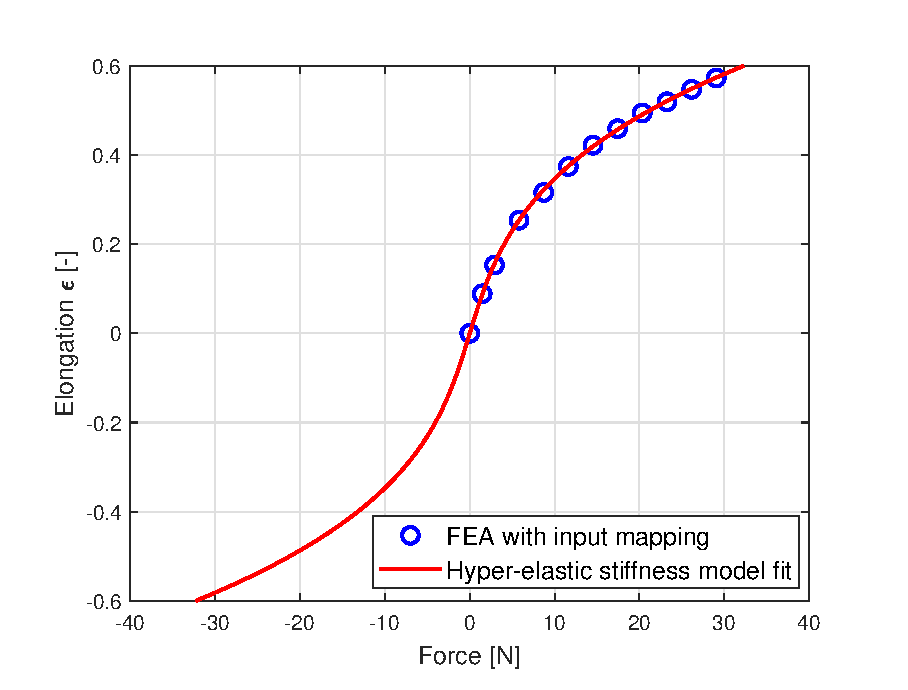
\includegraphics[width=\textwidth]{Figures/Chapter3/mappedforcevselongation.eps}
        \caption{Fitted stiffness model for elongation.}
        \label{fig3:elongvsforce}
    \end{minipage}\hfill
    \begin{minipage}{0.5\textwidth}
        \centering
        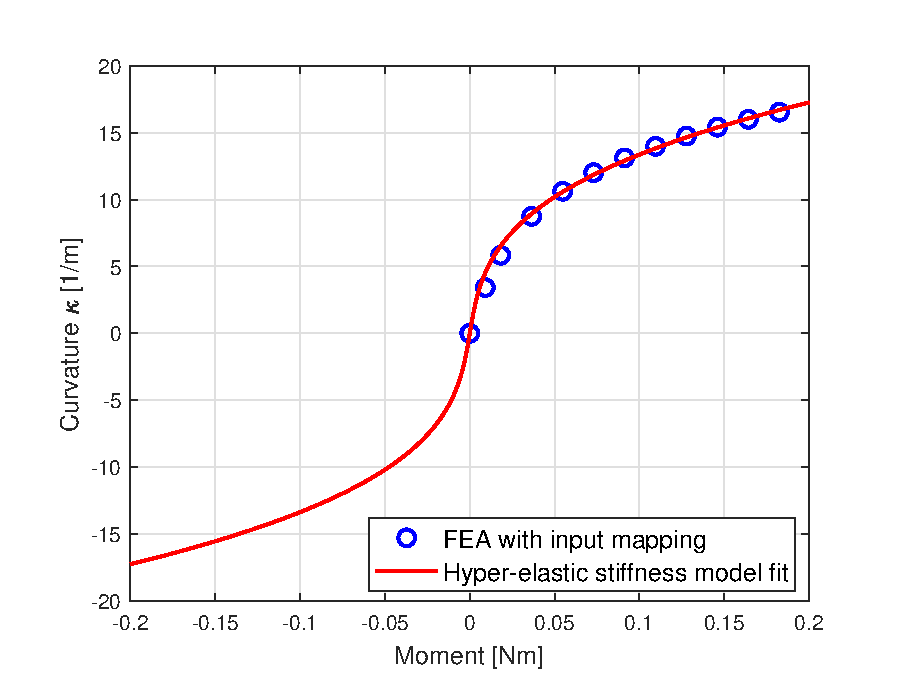
\includegraphics[width=\textwidth]{Figures/Chapter3/mappedmomentvscurvature.eps} 
        \caption{Fitted stiffness model for curvature.}
        \label{fig3:curvsmoment}
    \end{minipage}
\end{figure}